\chapter{Evaluation}\label{cha:evaluation}

Envoy is designed based on assumptions about a platform that does not yet exist. This limits how the system can be evaluated in two ways. The first is scalability. While common bottlenecks can be avoided and the architecture examined for potential scalability limitations, a system without a large-scale implementation can never be fully tested for issues that only appear at large scales. The best that can be achieved is to identify the most likely sources of problems and extrapolate the results of testing on a smaller scale. The architecture can also be evaluated against assumptions about the workloads it is intended to support, which leads to the second limitation: workloads cannot be accurately forecast. Predicting and simulating client access patterns is a difficult problem even for existing environments \cite{ganger95}, and the problem is amplified for service clusters. As a general purpose platform, service clusters are intended to support a wide range of existing workloads and to enable a flourishing ecosystem of computation services that create entirely new workloads. The design and the evaluation must necessarily rely on assumptions about how the system will be used, and those assumptions limit the applicability of the results.

In this chapter I evaluate the Envoy prototype with three principal goals: to measure the impact of specific design choices, including the basic distributed organisation and cache layout, to assess the scalability of the system, and to evaluate Envoy's ability to support the types of workloads expected in service clusters.

\section{Methodology}

The absence of a realistically sized service cluster limits the scope of system-level testing and the usefulness of many application-level results. The performance side-effects of interacting components and the access patterns of different clients are particularly difficult to predict. The performance characteristics of the storage layer depend on design elements and implementation choices beyond the scope of this dissertation. These factors combined with the poor public availability of many comparable systems limit direct comparisons to previous work.

Building and evaluating a prototype of the Envoy file system is not a futile exercise, however. The artefact may reveal little about real-world usage and behaviour, but measuring it can still do much to justify or condemn the design. This section starts by outlining assumptions about service clusters that influence the design, how the design reflects them, and how measuring the prototype helps to evaluate the decisions made. It concludes with a description of the testing environment and the benchmarks used.

\subsection{Assumptions and goals}

Envoy's success in achieving its stated goals is evaluated partly through argument and comparison to other work as described in previous chapters. Other aspects can be tested directly on a small installation and the results extrapolated to larger configurations. While not comprehensive, this approach is consistent with Envoy's role as one part of a complete service cluster environment. Further research and engineering will be necessary before service clusters can be fully evaluated on their own merits. Some of the assumptions that underpin them can be tested directly, while others must rest on arguments and an appeal to past and future work.

\subsubsection{Independent clients}

Though efficient sharing is important, individual clients accessing unshared data dominates most workloads. Even when data sets overlap, time may divide access from different clients, effectively yielding exclusive access that is transferred from one client to the next over time. Envoy seeks to capture these patterns by subdividing territories to distribute file ownership and control, and by dynamically updating the boundaries over time in response to changing usage. When this is successful, or when access to was exclusive in the first place, Envoy resembles a simple client-server system serving files from an administrative virtual machine to a client virtual machine on the same host.

Since one of Envoy's goals is to create this intra-host configuration whenever possible, the evaluation starts by considering system performance under this circumstance. Maximising raw performance is not the focus of the prototype implementation, but comparing it to systems with a similar topology creates baseline expectations for a production system, and examining absolute performance figures helps confirm the sanity of the overall design.

\secref{sec:independent-clients} evaluates the performance of Envoy as a file server within a single host. Composite performance numbers are compared to other client-server systems, and tests using different configurations help to demonstrate where performance costs are embedded in Envoy. In addition, performance for remote hosts is evaluated to show that the drive to localise traffic benefits performance as well as scalability.

\subsubsection{Shared images}

\secref{sec:shared-images} turns the evaluation to shared data. The emphasis of this section is not on performance---which is dependent largely on runtime topology as evaluated in \secref{sec:independent-clients} and the quality of the implementation---but rather on the behaviour of the system under shared workloads. In effect, \secref{sec:shared-images} evaluates Envoy's ability to localise traffic, and \secref{sec:independent-clients} explores the benefits and costs that result from its success or failure.

Some aspects of Envoy's dynamic behaviour cannot be adequately tested in the limited environment available for this evaluation. The Envoy design prizes simplicity and stability in the layout of territories, both to simplify testing and recovery, and to encourage cache sharing even in the presence of runtime conflicts. The latter goal is achieved by delaying territory transfers until traffic is clearly dominated by a remote participant or until a more slight imbalance has persisted for a longer period of time. Resisting change allows the cache on the owning host to serve all participants at the expense of a network hop from the remote client to the envoy. Rearranging boundaries more eagerly may reduce network hops, but it creates some migration latency and the new host may have to prime its cache before service can resume at full speed.

While the parameters controlling dynamic behaviour can be configured, the ideal balance of stability and layout optimality can only be adequately determined with realistic workloads. Oscillating demand could be best handled by reacting quickly and varying the territory layout in lock-step with traffic changes, or being reluctant to change in order to maximise cache efficacy on one of the hosts may prove better. In the absence of a larger test system and realistic workloads to evaluate specific parameters, this evaluation relies on artificial traffic loads that can be controlled and varied to test the response of the system.

\subsubsection{Scalability}

Envoy's scalability is not evaluated directly. To do so convincingly would require a large cluster with a diverse client base, and direct testing on a reduced scale would prove little. The presumed scalability of the system depends on successfully localising as much traffic as possible. If all requests are satisfied by the same physical machine that hosts the client, then a cluster's capacity to host clients grows linearly with the number of machines added to the system. If most requests are handled locally and neighbouring hosts are consulted mainly to resolve runtime conflicts, then scalability is limited primarily by the degree of runtime sharing. Envoy's goal of scalability is based on a design that attempts to approximate that limit.

The storage layer is another source of traffic and inter-host dependence, but it is not fully specified in this work and cannot be evaluated fairly. A large persistent cache on each host reduces the direct load on the storage layer just as it did for AFS \cite{satyanarayanan85}, but by coupling storage nodes with clients hosts and using switched networking, the overall transaction capacity of the storage layer should scale with the number of hosts anyway, and the number of hosts limits the number of clients. The systems considered in \secref{sec:storage-layer-systems} have already demonstrated the scalability of similar storage architectures; conflict management and the coordination of metadata differentiate each system, but in Envoy that burden is not left to the storage layer.

\subsubsection{Features}

Rapid and inexpensive deployment of services requires support from the file system, and is one of the principal motivations for Envoy. The demands of a software ecosystem are difficult to predict, and Envoy's suitability for this environment is likewise difficult to assess. Features allowing rapid cloning and snapshots of file system images contribute to the flexibility of service clusters and are intended to promote the use of commodity software, but their actual impact in a production system is a matter of speculation. The speed with which images can be cloned and new services launched is measured in \secref{sec:image-operations}.

\subsection{Test environment}

\subsubsection{Hardware}

\subsubsection{Benchmarks}

Linux source tree: stats about it

untar -- write test

tar > /dev/null -- read test

rsync -- 2nd read test

Bonnie: info about it

\section{Independent clients}\label{sec:independent-clients}

Much of the complexity in distributed file system design is related to data sharing, but sharing is less common than individual clients accessing private data. A service derived from a stand-alone machine typically requires a private boot image, and lightweight fork operations in Envoy encourage the cloning of entire images for private use by related and unrelated service instances.

To succeed as a distributed file system on a large scale, Envoy must provide a useful service to isolated clients that obviates the need for additional storage services for most clients. While there is no technical or administrative distinction between private and shared images, Envoy's design and runtime behaviour under these two conditions can be evaluated separately. This section focuses on Envoy's performance and behaviour in the absence of sharing.

\subsection{Performance}

The prototype is not optimised, and absolute performance is not the focus of this evaluation. Nevertheless, it is helpful to establish baseline performance numbers to show that Envoy is viable as a file system. For context, the results are compared to \texttt{npfs}, a multi-threaded userspace 9p server, and \texttt{unfsd}, a single-threaded userspace NFS server. Userspace servers have additional overhead when compared to kernel implementations, but the penalty is assumed to be similar for all of the implementations tested. Standard benchmarks do a poor job of isolating the costs involved in Envoy's data paths, and most of the evaluation in this chapter eschews them in favour of more controlled tests, but this section starts with the Bonnie benchmark to provide some raw performance figures comparable to those from other systems.

\begin{figure}[t]
\centering
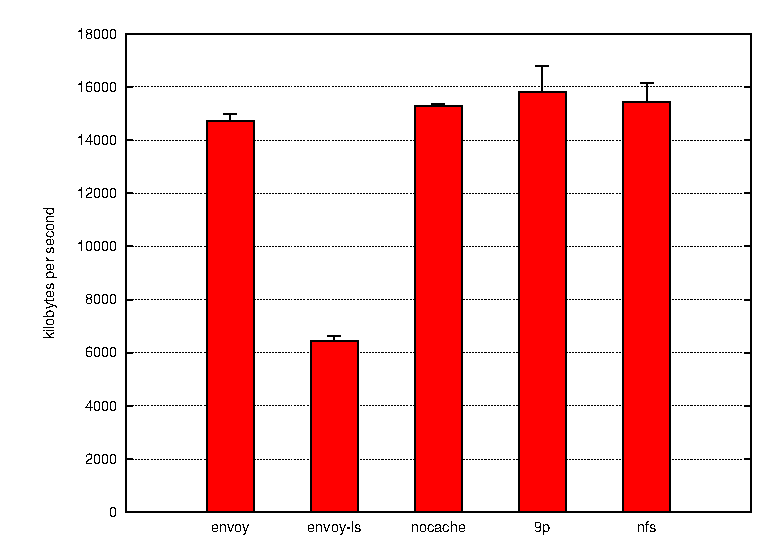
\includegraphics[width=\figwidth]{figures/bonnie-druid1-write}
\caption[Bonnie benchmark results for block writes]{Bonnie benchmark results for block writes on a 2~GB dataset. Results for Envoy, Envoy using a local storage server instance, Envoy with no persistent cache, a userspace 9p server, and a userspace NFS server are compared. Error bars show the standard deviation over ten runs.}
\label{fig:bonnie-druid1-write}
\end{figure}

\figref{fig:bonnie-druid1-write} shows the block write results of the Bonnie benchmark on a 2~GB dataset. Envoy is competitive with the 9p and NFS servers, despite writing to two storage servers and the local persistent cache. Bonnie does not force a sync after writing, so this represents a conservative result for Envoy. When the write is complete, Envoy has flushed the data to two storage servers and can tolerate a node failure without loss, while the 9p and NFS servers both have a dirty cache on a single node with no replicas.

For sustained writes, the disk is the primary bottleneck, as demonstrated by the result labelled \emph{envoy-ls}, which has one of the two storage servers on the same machine as the envoy. In this case, data must be written twice using the same disk, once for the cache and a second time for the storage instance. In addition, the in-memory cache is split between the two functions, cutting its effective size in half. The \emph{nocache} figure is an Envoy server with the persistent cache disabled, a change that has little effect in this test because the writes are performed in parallel on each node.

Envoy nodes all host storage servers, and it is reasonable to assume that each node generates a similar amount of traffic on average. Storage is distributed throughout the cluster, so it is less likely that a node with a write-heavy client will also host storage for other write-heavy clients at the same time; envoy-ls represents a worst-case scenario rather than a common case.

\begin{figure}[t]
\centering
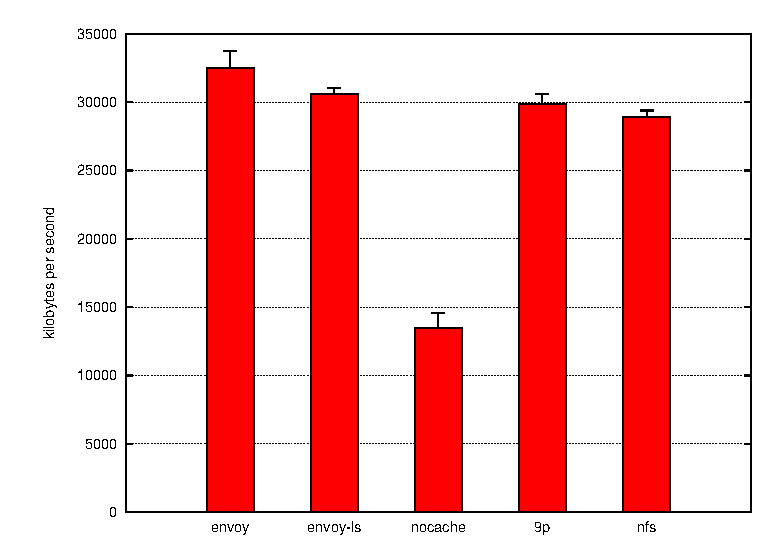
\includegraphics[width=\figwidth]{figures/bonnie-druid1-read}
\caption[Bonnie benchmark results for block reads]{Bonnie benchmark results for block reads on a 2~GB dataset. Results for Envoy, Envoy using a local storage server instance, Envoy with no persistent cache, a userspace 9p server, and a userspace NFS server are compared. Error bars show the standard deviation over ten runs.}
\label{fig:bonnie-druid1-read}
\end{figure}

\figref{fig:bonnie-druid1-read} shows the block read results from the same benchmark. Bonnie's test uses a single file, so the Envoy servers are reading data from a single file in the persistent cache. All of the tests except nocache involve transfers from a single file in one VM to a client in another VM, with similar overall results. As in the write tests, the results are dominated by disk speeds.

With no persistent cache, Envoy must fetch each block from one of the storage servers. The prototype limits files to one outstanding transaction each, so parallelism is not exploited in this test, and requests are randomly distributed to the two storage servers, so neither ends up with a sequential read through the entire file. A more sophisticated storage layer would likely reduce the penalty of omitting the persistent cache, but in normal operation most data is expected to be in the persistent cache anyway.

\begin{figure}[t]
\centering
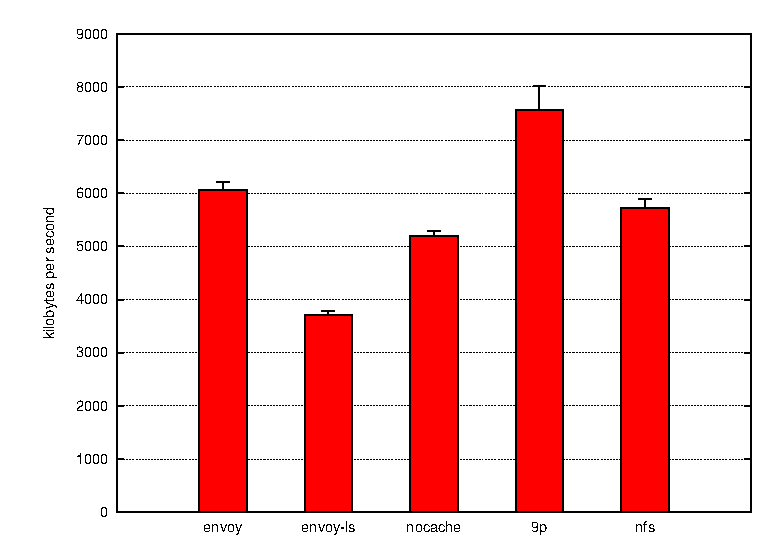
\includegraphics[width=\figwidth]{figures/bonnie-druid1-rewrite}
\caption[Bonnie benchmark results for block re-writes]{Bonnie benchmark results for block re-writes on a 2~GB dataset. Each block in the dataset is read, modified, and written back in sequence. Results for Envoy, Envoy using a local storage server instance, Envoy with no persistent cache, a userspace 9p server, and a userspace NFS server are compared. Error bars show the standard deviation over ten runs.}
\label{fig:bonnie-druid1-rewrite}
\end{figure}

Bonnie's re-write test reads the same file in sequence, writing back a change to each block as it is encountered, with results displayed in \figref{fig:bonnie-druid1-rewrite}. The Envoy results reflect the write penalty for a local storage server and the read penalty for no persistent cache, with no surprises. Envoy lags behind 9p in this test, probably because the read is done from the persistent cache, but the write requires each storage server to seek the correct position in the file for each write afterward. Unlike the write test, where the three disks work in parallel, this test forces a seek and read from one disk, followed by a seek and write to all three. For the second seek, the 9p server and the persistent cache are more likely to find the disk head in the right place than the storage servers, which omitted the first seek.

The poor showing from NFS relative to 9p is due to an artifact in the test that interacts with the client-side cache. The rewrite test is preceded by the write test with no explicit \texttt{sync} operation to flush the write cache to disk. All of the re-write tests start with a dirty cache, but NFS adds the client's cache to that of the server, leaving more writes from the previous test that are billed to the current one.

The results from testing with Bonnie show Envoy to be competent at serving files in a simple client-server configuration between two virtual machines. Results are comparable to a simple 9p or NFS server for operations on datasets larger than the in-memory cache size. In these tests, the speed of the disk appears to be the primary bottleneck, which is the expected result for basic operations involving bulk data transfer with few metadata operations. The remainder of this section explores the results in more detail to reveal the effect that the network and virtual machine architecture have on performance and how caching, both in-memory and on-disk, influences performance.

\subsection{Architecture}\label{sec:architectural-costs}

An important goal of the Envoy design is to localise data and metadata control when possible, and minimise the involvement of disinterested nodes when not possible. Private images are always controlled by the envoy instance on the same machine as the client using it, and territories in shared images are managed by the most active participant. Besides reducing collateral impact in a bid to improve scalability, localising control and caching has direct performance benefits for clients.

As described in \secref{sec:data-paths}, requests follow one of several paths to completion depending on whether or not the required data is cached and whether ownership is local or remote. The impact of network and virtual machine layout is measured here, with four layouts. \emph{druid-0} is an administrative virtual machine that hosts all server processes, and owns all territories in the case of Envoy. \emph{skiing-0} is an administrative VM on a different machine, hosting Envoy server processes but no others. \emph{druid-1} and \emph{skiing-1} are client VMs on the two machines. These tests focus on hot cache results to prevent disk access time from masking other sources of overhead.

For the 9p and NFS results, druid-0 acts as the server in all instances, and results are included for all four client locations. Envoy clients attach to their local envoy instance in each case, so for clients on skiing, all requests are forwarded on to the envoy instance running on druid-0.

\begin{figure}[t]
\centering
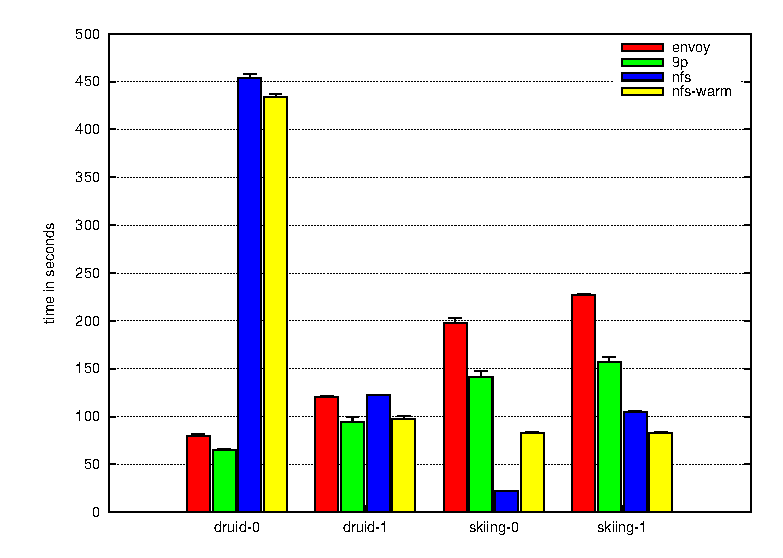
\includegraphics[width=\figwidth]{figures/arch-tar-hot}
\caption[\texttt{tar} benchmark results with hot cache]{Time to \texttt{tar} the Linux kernel source tree with a hot cache over various data paths. NFS results are included for a hot client-side cache and for a hot server-side cache only (labelled nfs-warm). Error bars show the standard deviation over ten runs.}
\label{fig:arch-tar-hot}
\end{figure}

\figref{fig:arch-tar-hot} shows the time required to \texttt{tar} the Linux kernel source tree from each client location with a hot cache. In each case, the file data is available from the buffer cache of druid-0, so the differences are largely due to network, protocol, and implementation overhead. The Envoy and 9p results show a significant difference between druid-0 and druid-1 results, which comes from the virtual network device that connects the two VMs. Much of this overhead could be eliminated through a Xen-specific transport between the VMs combined with optimisations in the 9p driver to eliminate data copying, as suggested in \secref{sec:data-paths-read}.

Envoy is consistently slower in this test than in the Bonnie read test, which measured bulk operations from a single file. The \texttt{tar} test exercises metadata operations much more heavily, which exposes the extra overhead of a prototype-quality implementation of Envoy. For the skiing-0 and skiing-1 results, requests are considered and forwarded at the skiing-0 envoy instance, so overhead is inherent to the design. For druid-0 and druid-1, however, both 9p and Envoy are using the same protocol to deliver the same data across the same network paths, and the data is coming from the buffer cache in each instance. Optimisation of the prototype would probably result in something closer to parity between these results.

The NFS results for druid-0 are an exception caused by the client-side cache. Because the client and server must compete for cache space, the cache is not sufficient to hold the file tree and disk access is required. While seemingly an unfair circumstance for the NFS results, this result is included to illustrate the benefit of shared caching. Allowing a larger unified cache on each host instead of having each client provide its own smaller cache reduces this kind of cache duplication and increases the effective cache space available cluster-wide. While the local cache can improve performance, it can also cause more disk access and reduce both performance and the overall transaction capacity of the cluster.

A second anomaly caused by the client-side cache is the result for skiing-0, where the entire file tree fits in the client-side cache. The displayed result is only applicable when the test is repeated within the 30-second window in which the Linux NFS client considers data valid. The test completes in an average of 22.38 seconds and makes this possible, but if a delay is introduced between each iteration, the average time nearly doubles to 44.05 as each cache entry must be validated against the server.

\begin{figure}[t]
\centering
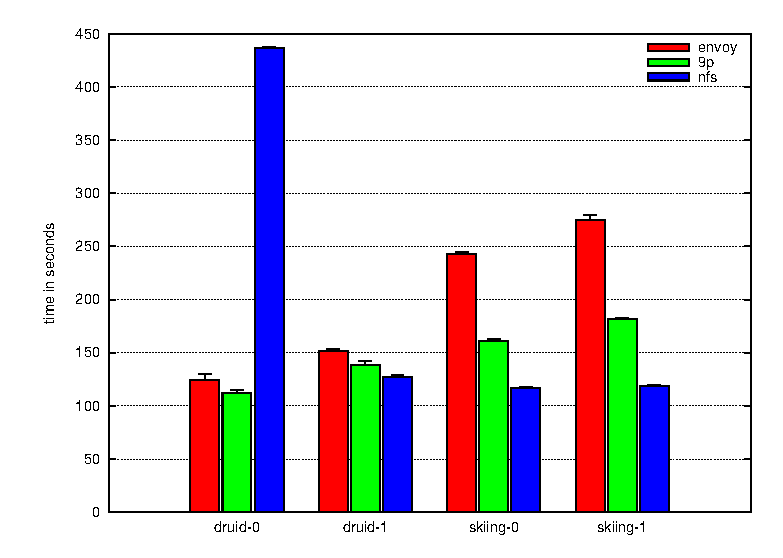
\includegraphics[width=\figwidth]{figures/arch-tar-warm}
\caption[\texttt{tar} benchmark results with a warm cache]{Time to \texttt{tar} the Linux kernel source tree from the persistent cache (for Envoy), with the in-memory cache cold for all servers. Error bars show the standard deviation over ten runs.}
\label{fig:arch-tar-warm}
\end{figure}

\figref{fig:arch-tar-warm} supplements these results with the same tests with the in-memory cache flushed before each iteration. Data is resident in the persistent cache in the case of Envoy, so for each of the three servers the data is coming from the same disk. NFS suffers from the same double-buffering issue on druid-0, but otherwise its client-side cache proves very helpful for the metadata-intensive operations in this test. This is clearest in the jump to a remote machine, where 9p must consult a remote server for many operations that are absorbed by the client-side cache in NFS. If the optimisations already suggested prove insufficient, an approach like that of NFSv4---where a limited token-passing scheme lets clients access unshared files without fear of conflicts but reverts control of shared files to the server \cite{shepler}---may be useful for Envoy, allowing it to retain strong consistency guarantees while allowing local caching for unshared files. Testing with a representative workload on an optimised implementation of Envoy would better inform such a choice.

These tests do show a clear performance benefit to coupling control of territories with the clients that use them, particularly in the difference between Envoy results for druid-1 and skiing-1. Comparing the two graphs also shows that Envoy is faster serving warm data controlled by the same machine than hot data from a remote machine, suggesting that territory boundaries can be relatively fluid without destroying performance.

\begin{figure}[t]
\centering
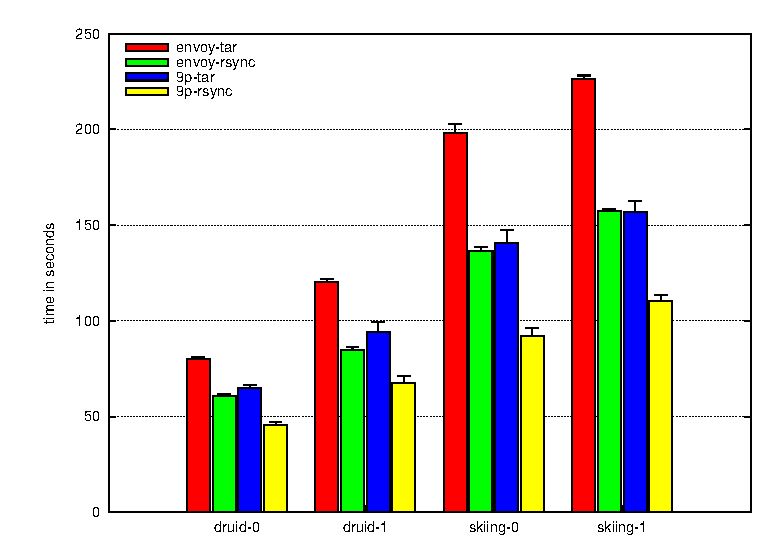
\includegraphics[width=\figwidth]{figures/arch-rsync-tar-hot}
\caption[\texttt{tar} and \texttt{rsync} benchmark results with a hot cache]{Time to read the Linux kernel source tree using \texttt{tar} and \texttt{rsync} after priming the in-memory cache with all file data. Error bars show the standard deviation over ten runs.}
\label{fig:arch-rsync-tar-hot}
\end{figure}

\figref{fig:arch-rsync-tar-hot} compares using \texttt{tar} and \texttt{rsync} to read the Linux kernel source tree from cache using Envoy and 9p. \texttt{rsync} reads asynchronously from multiple files at one time, whereas \texttt{tar} reads one file to completion before starting the next. The increase in time required for both tests between druid-1 and skiing-1---which are the two important client locations---is quite consistent, inviting a cautious comparison between the two. Envoy sees a time increase of 88\% for \texttt{tar} and 85\% for \texttt{rsync}, while 9p sees 67\% for \texttt{tar} and 63\% for \texttt{rsync}. It appears that forwarding skiing-1 requests through the envoy on skiing-0 exacts an overhead of roughly 20\% compared to sending requests directly to druid-0.

Envoy uses the 9p protocol to connect to clients, and it also uses an extended version of it between envoy instances. Comparisons between Envoy and a simple 9p server using similar data paths and cached results demonstrates that the 9p server is consistently faster, but performance degrades at a similar rate for both systems as obstacles are introduced to the data paths. The 9p server passes most requests directly to the file system, while Envoy is a more complex system that tracks additional state and offers more features. Nevertheless, the correlation between the two optimistically suggests that the Envoy prototype could optimised to a performance level close to that of the 9p server without introducing any architectural changes. A roughly 20\% overhead beyond network costs for remote transactions is imposed by the forwarding system, but this is a reasonable tradeoff for simplified recovery and transparent territory migrations that the Envoy architecture enables.

\subsection{Cache}

In addition to the data paths imposed by the architecture, Envoy requests interact with different cache states. When the cache is \emph{hot}, data is available from the in-memory cache on the envoy that owns the relevant territory. A \emph{warm} cache holds data in the local on-disk cache, but not the in-memory cache. When data must be retrieved from the storage layer, the cache is said to be \emph{cold}, and for all tests the storage servers themselves were restarted and data partitions remounted to empty in-memory buffers.

For all Envoy tests, the server was restarted between each iteration, reseting the server's internal state. For both hot and warm cache tests, the server must initially validate cached objects against the storage servers, but can then proceed to use them from the local cache. Testing found this to have little effect on the results, so all figures presented here use the more conservative method.

\section{Shared images}\label{sec:shared-images}



\subsection{Territory migration}

cost of transferring state

two machines with kernel in hot cache, do read test while transferring ownership back and forth between them

\subsection{Dynamic behaviour}

Test dynamic territory management, less about performance than behaviour

probabilistic traffic driven to overlapping areas

shared image with (independent) home directories

2 log files in one directory

producer-consumer

\subsubsection{Sharing application}
something that shares in a complex but predictable fashion

\section{Image operations}\label{sec:image-operations}

Service clusters must be able to easily manipulate file system images to achieve their promised flexibility. Providing templates with commodity software and allowing clients to easily clone and customize them makes service instantiation a relatively lightweight operation. When combined with functionality in the virtual machine monitor to suspend, clone, and resume running services, this could allow rapid instantiation of common services. Envoy provides support for rapid forking of file system images, along with the ability to take snapshots of active images. This section measures the performance of these two management operations, along with the time and space required to deploy new services.

\subsection{Forks}

New images can be created from scratch, or they can be forked from an existing image. Forks always start from a snapshot of an existing image, and snapshots are always read-only. With the copy-on-write mechanism described in \secref{sec:snapshots}, this makes forks a fast and efficient operation. Even if the template snapshot is in active use, only the root of the image needs to be copied to isolate the new image from the old.

The time required to fork an image was measured in two ways. In the first, the server was instrumented to record the time spent completing the operation. Over fifty iterations, the average fork took 339~$\mu$seconds with a standard deviation of 32~$\mu$seconds. Over the same fifty iterations, the client VM observed the time required to fork the template and create a new file in the new image. \texttt{/usr/bin/time} reported 10~milliseconds for each iteration, which corresponds to its timer resolution.

\subsection{Snapshots}

Forking an existing template is fast because few operations are involved. Snapshots can be taken of active images, which may involved cloning storage objects as well as copying runtime state. If an image has been divided into multiple territories, the snapshot operation will span multiple envoy instances and will required cloning a path from the root of the image to each territory root, as discussed in \secref{sec:snapshots}. Forking an active image also involves taking a snapshot and then performing a fork operation, so dividing an active system is dependent on the snapshot mechanism as well.

In the simple case, snapshots are nearly as fast as forks. When an image is inactive, taking a snapshot requires cloning the root, adding the new snapshot to the parent directory, and updating the link to the active view of the image. Over fifty iterations, an instrumented server reported an average of 1258~$\mu$seconds per snapshot with a standard deviation of 108~$\mu$seconds.

To evaluate more complex snapshot cases, a tree of territories involving three machines was created. Control of a Linux kernel source tree was divided such that every directory was the root of a territory owned by a different envoy than its parent, i.e., every territory was forced to cede control of subdirectories equally between the other two servers. druid-0 was the root server and hosted 439 territories, skiing-0 hosted 421, and moonraider-0 hosted 379 territories, for a total of 1239 territories. This is far beyond what one would expect in a normal deployment for a single image, but serves to exercise the snapshot mechanism under extreme conditions.

After constructing the territory tree, fifty snapshots were taken of the kernel image in an average of 13.71~seconds each with a standard deviation of 3.13~seconds, or approximately 11.1~milliseconds per territory in the tree. Most of this time was spent cloning objects to ensure that the root of each territory was writable in the active image after the snapshot completed. Under Envoy's consistency semantics, this requires submitting changes to the storage servers before considering the operation complete, but not flushing their buffers to disk. If the snapshots are done in rapid succession, the storage server buffers cannot absorb the traffic and disk write times increase the time. After a warmup run of several snapshots, fifty more were done without pause in an average of 73.13~seconds each with a standard deviation of 26.8~seconds, or approximately 59~milliseconds per territory. The high variability comes from the lack of coordination between the client operations and the buffer cache on the storage serves.

The snapshot timings reflect a combination of network messages, internal state updates, and storage object updates. The bulk of the time is spent doing storage object updates, though this is not measured directly. To approximate this, another operation can be measured that performs similar state updates and has the same network message profile, but does not involve updating storage objects. Renaming the root directory requires recursively notifying child territories of the pathname change, which makes it a suitable choice. Fifty such operations complete in an average of 96.7~milliseconds each with a standard deviation of 1.09~milliseconds, approximately 78~$\mu$seconds per territory.

\subsection{Service deployment}

Besides making service deployment quick, an important goal of snapshot and fork operations using copy-on-write is to encourage the use of commodity software and exploit the redundancy that results. Objects inheritet from a common template or a previous snapshot can be read by any envoy without coordination, as higher-level semantics guarantee that the object will not be modified again. This allows cache sharing for read-only objects between unrelated services. Besides cutting down the cache required on a given node, this makes it likely that common template objects will already be loaded into the persistent cache of typical nodes, allowing the most common objects to be served locally and reducing the cluster-wide load on storage servers.

\begin{table}[t]
\begin{center}
\begin{tabular}{l|>{\ttfamily}l>{\ttfamily}l}
                        & \textrm{Cold cache} & \textrm{Hot cache} \\ \hline
Client requests/bytes   & 70,016/1,264,742    & 71,648/1,296,578 \\
Client responses/bytes  & 70,016/79,457,018   & 71,648/81,323,281 \\
Storage requests/bytes  & 2,764/288,858       & 2,059/285,429 \\
Storage responses/bytes & 2,764/17,476,789    & 2,059/675,196
\end{tabular}
\end{center}
\caption[Service deployment storage overlap figures]{Messages and bytes transferred when a virtual machine boots from an Linux template image. The first was booted with a cold cache, and the second after restarting Envoy but not clearing the in-memory or on-disk cache. In the hot cache case, objects had to be validated against the storage server because of the server restart, hence the similar message counts, but data could be retrieved from the cache.}
\label{tab:deployment-stats}
\end{table}

To measure this effect, a template image was prepared with SUSE Linux Enterprise Server~10, and a virtual machine booted from a fork of this image with a cold cache. Another VM booted from a second fork of the image, this time with the cache primed from the first one. Boot times as measured with a stopwatch were about 50~seconds in either case, with the hot cache a few seconds faster (compared to about 30~seconds when booting from a local partition).

\tabref{tab:deployment-stats} shows the results collected by an instrumented version of Envoy. The server was restarted between tests, so the hot cache results include message traffic to validate cached objects with the storage servers. Booting the second image pulled less than 4\% of the bytes retrieved from the storage layer when starting the first image, showing a heavy overlap between read-only data in the two instances. Combined with the lightweight snapshot and fork operations, this suggests that service instances can be created and deployed quickly and with little impact beyond the local machine.

\section{Summary}
